%%%%%%%%%%%%%%%%%%%%%%%%%%%%%%%%%%%%%%%%%
% Arsclassica Article
% LaTeX Template
% Version 1.1 (10/6/14)
%
% This template has been downloaded from:
% http://www.LaTeXTemplates.com
%
% Original author:
% Lorenzo Pantieri (http://www.lorenzopantieri.net) with extensive modifications by:
% Vel (vel@latextemplates.com)
%
% License:
% CC BY-NC-SA 3.0 (http://creativecommons.org/licenses/by-nc-sa/3.0/)
%
%%%%%%%%%%%%%%%%%%%%%%%%%%%%%%%%%%%%%%%%%

%----------------------------------------------------------------------------------------
%	PACKAGES AND OTHER DOCUMENT CONFIGURATIONS
%----------------------------------------------------------------------------------------

\documentclass[
10pt, % Main document font size
a4paper, % Paper type, use 'letterpaper' for US Letter paper
oneside, % One page layout (no page indentation)
%twoside, % Two page layout (page indentation for binding and different headers)
headinclude,footinclude, % Extra spacing for the header and footer
BCOR5mm, % Binding correction
]{scrartcl}


%%%%%%%%%%%%%%%%%%%%%%%%%%%%%%%%%%%%%%%%%
% Arsclassica Article
% Structure Specification File
%
% This file has been downloaded from:
% http://www.LaTeXTemplates.com
%
% Original author:
% Lorenzo Pantieri (http://www.lorenzopantieri.net) with extensive modifications by:
% Vel (vel@latextemplates.com)
%
% License:
% CC BY-NC-SA 3.0 (http://creativecommons.org/licenses/by-nc-sa/3.0/)
%
%%%%%%%%%%%%%%%%%%%%%%%%%%%%%%%%%%%%%%%%%

%----------------------------------------------------------------------------------------
%	REQUIRED PACKAGES
%----------------------------------------------------------------------------------------

\usepackage[
nochapters, % Turn off chapters since this is an article        
beramono, % Use the Bera Mono font for monospaced text (\texttt)
eulermath,% Use the Euler font for mathematics
pdfspacing, % Makes use of pdftex’ letter spacing capabilities via the microtype package
dottedtoc % Dotted lines leading to the page numbers in the table of contents
]{classicthesis} % The layout is based on the Classic Thesis style

\usepackage{arsclassica} % Modifies the Classic Thesis package

\usepackage[T1]{fontenc} % Use 8-bit encoding that has 256 glyphs

\usepackage[utf8]{inputenc} % Required for including letters with accents

\usepackage{graphicx} % Required for including images
\graphicspath{{Figures/}} % Set the default folder for images

\usepackage{enumitem} % Required for manipulating the whitespace between and within lists

\usepackage{lipsum} % Used for inserting dummy 'Lorem ipsum' text into the template

\usepackage{subfig} % Required for creating figures with multiple parts (subfigures)

\usepackage{amsmath,amssymb,amsthm} % For including math equations, theorems, symbols, etc

\usepackage{varioref} % More descriptive referencing
\usepackage{color,listings}
\usepackage{csquotes}
\usepackage{textcomp}
\usepackage{tcolorbox}
\usepackage{smartdiagram}


%----------------------------------------------------------------------------------------
%	THEOREM STYLES
%---------------------------------------------------------------------------------------

\theoremstyle{definition} % Define theorem styles here based on the definition style (used for definitions and examples)
\newtheorem{definition}{Definition}

\theoremstyle{plain} % Define theorem styles here based on the plain style (used for theorems, lemmas, propositions)
\newtheorem{theorem}{Theorem}

\theoremstyle{remark} % Define theorem styles here based on the remark style (used for remarks and notes)

%----------------------------------------------------------------------------------------
%	HYPERLINKS
%---------------------------------------------------------------------------------------

\hypersetup{
%draft, % Uncomment to remove all links (useful for printing in black and white)
colorlinks=true, breaklinks=true, bookmarks=true,bookmarksnumbered,
urlcolor=webbrown, linkcolor=RoyalBlue, citecolor=webgreen, % Link colors
pdftitle={NodeRED Project Report}, % PDF title
pdfauthor={Tanmaya Mahapatra}, % PDF Author
pdfsubject={Yearly Report}, % PDF Subject
pdfkeywords={}, % PDF Keywords
pdfcreator={pdfLaTeX}, % PDF Creator
pdfproducer={LaTeX with hyperref and ClassicThesis} % PDF producer
}

\lstset{ %
  upquote=true,
  backgroundcolor=\color{white},   % choose the background color; you must add \usepackage{color} or \usepackage{xcolor}; should come as last argument
  basicstyle=\footnotesize,        % the size of the fonts that are used for the code
  breakatwhitespace=false,         % sets if automatic breaks should only happen at whitespace
  breaklines=true,                 % sets automatic line breaking
  captionpos=b,                    % sets the caption-position to bottom
  commentstyle=\color{green},    % comment style
  deletekeywords={...},            % if you want to delete keywords from the given language
  escapeinside={\%*}{*)},          % if you want to add LaTeX within your code
  extendedchars=true,              % lets you use non-ASCII characters; for 8-bits encodings only, does not work with UTF-8
  frame=single,	                   % adds a frame around the code
  keepspaces=true,                 % keeps spaces in text, useful for keeping indentation of code (possibly needs columns=flexible)
  keywordstyle=\color{blue},       % keyword style
  language=SQL,                 % the language of the code
  morekeywords={*,...},            % if you want to add more keywords to the set
  numbers=left,                    % where to put the line-numbers; possible values are (none, left, right)
  numbersep=5pt,                   % how far the line-numbers are from the code
  numberstyle=\tiny\color{gray}, % the style that is used for the line-numbers
  rulecolor=\color{black},         % if not set, the frame-color may be changed on line-breaks within not-black text (e.g. comments (green here))
  showspaces=false,                % show spaces everywhere adding particular underscores; it overrides 'showstringspaces'
  showstringspaces=false,          % underline spaces within strings only
  showtabs=false,                  % show tabs within strings adding particular underscores
  stepnumber=2,                    % the step between two line-numbers. If it's 1, each line will be numbered
  stringstyle=\color{green},     % string literal style
  tabsize=2,	                   % sets default tabsize to 2 spaces
  title=\lstname                   % show the filename of files included with \lstinputlisting; also try caption instead of title
} % Include the structure.tex file which specified the document structure and layout

\hyphenation{Fortran hy-phen-ation} % Specify custom hyphenation points in words with dashes where you would like hyphenation to occur, or alternatively, don't put any dashes in a word to stop hyphenation altogether

%----------------------------------------------------------------------------------------
%	TITLE AND AUTHOR(S)
%----------------------------------------------------------------------------------------

\title{\spacedallcaps{Distance Based Application Trigger}} % \spacedallcaps The article title

\author{\small{Mehdi Yosofie, Philipp Schlieker}} %   The article author(s) - author affiliations need to be specified in the AUTHOR AFFILIATIONS block

\date{\today} % An optional date to appear under the author(s)

%----------------------------------------------------------------------------------------

\begin{document}

%----------------------------------------------------------------------------------------
%	HEADERS
%----------------------------------------------------------------------------------------

\renewcommand{\sectionmark}[1]{\markright{\spacedlowsmallcaps{#1}}} % The header for all pages (oneside) or for even pages (twoside)
%\renewcommand{\subsectionmark}[1]{\markright{\thesubsection~#1}} % Uncomment when using the twoside option - this modifies the header on odd pages
\lehead{\mbox{\llap{\small\thepage\kern1em\color{halfgray} \vline}\color{halfgray}\hspace{0.5em}\rightmark\hfil}} % The header style

\pagestyle{scrheadings} % Enable the headers specified in this block

%----------------------------------------------------------------------------------------
%	TABLE OF CONTENTS & LISTS OF FIGURES AND TABLES
%----------------------------------------------------------------------------------------

\maketitle % Print the title/author/date block

\setcounter{tocdepth}{2} % Set the depth of the table of contents to show sections and subsections only

\tableofcontents % Print the table of contents

%\listoffigures % Print the list of figures

%\listoftables % Print the list of tables

%----------------------------------------------------------------------------------------
%	ABSTRACT
%----------------------------------------------------------------------------------------

\section*{Summary} % This section will not appear in the table of contents due to the star (\section*)

Context-awareness is an important issue in todays IoT world. Our project proposes a trigger that is activated based on the distance to a given object. In our scenario, we make us of the Bluetooth Low Energy (BLE) standard which allows the distance measurement between two objects. We use a BLE beacon together with the Bluetooth sensor of the smartphone in order to measure the distance. 


%----------------------------------------------------------------------------------------



%----------------------------------------------------------------------------------------
%	INTRODUCTION
%----------------------------------------------------------------------------------------

\section{Introduction}
The main idea of this project is to build an Android app that allows to trigger IoT devices based on position / distance thereby adding context-awareness. One standard way to do this, e.g. employed by IFTTT, is the use of GPS or the connectivity of WiFi networks. Both of these technologies allow for great radius but are quite limited in their accuracy. Thus, we propose to use Bluetooth Low Energy to estimate the distance. This is done by using a beacon that continously sends out a broadcast signal using Bluetooth. This signal is then received by a sensor which estimates the distance based on the signal strength. In our scenario we make us of a RaspberryPi as beacon and API. The sensor is then provided by an Android phone.


\section{Practical Applicability of the Project}
This type of project can be used in numerous scenarios. A few of which are the following:
\begin{enumerate}
\item 
	\begin{description}
	\item[Automatically Unlocking a door] Our prototype can be used to automatically unlock the front door of a house once the inhabitant arrives and thereby replacing the normal key. In contrast to WIFI the accuracy of BLE is high enough to \emph{only} keep the door unlocked while standing right next to it.
	\end{description}
	\item 
	\begin{description}
	\item[Switching Appliances] Another use case would be switching on and off appliances based on ones position in the room. One example would be a desk lamp which is switched on once the user is sitting at a desk and it is dark outside.
	\end{description}
	\item
	\begin{description}
	\item[Sensor for SmartHome Applications] Another use case is the use as a sensor for SmartHome Applications and thereby adding a wide range of possibilities. It is for example possible to switch on the light, adjust the room temperature and turn on music once a person enters a specific room.
	\end{description}
	\item
	\begin{description}
	\item[Preventing misuse of devices] Another option would be to prevent the misuse of devices by only allowing the invocation of a command when the person is in a specific location. This could be used by AirBnB to prevent guests from unlocking the front door when they are not there or by companies to enforce security policies.
	\end{description}
\end{enumerate}

\section{Conceptual Approach \& Architecture}

\noindent The used sensor is the Bluetooth sensor of an Android Smartphone. The Bluetooth Low Energy (BLE) Beacon is sending its signal constantly and periodically. The Smartphone (hold by a human) comes closer to the Beacon and detects the beacon. As soon as the beacon is detected by the smartphone (by the human), it sends (the human automatically sends) a HTTP request to our webserver to open the door/ to turn on the light. Our project architecture can be seen in figure \ref{fig:projectarchitecturefinal}.\\

\noindent We simulated the Beacon furthermore by a node.js application on PC. Thus, debugging and testing was faster and possible on every machine.\\

\noindent The HTTP request arrives on the webserver (a Raspberry Pi). The Rasberry Pi handles the request by activating the lamp or opening a lock via its GPIO.\\

\noindent The Raspberry can be reached over a public IP adress. We used Balena as deployment architecture for the Raspberry Pi. Balena \cite{balena} is a IoT cloud deployment platform where Balena images can be downloaded and flashed on the Raspberry. The image auto-pulls the code which the developer pushs on his git repository. On Balena, the Raspberry Pi gets a public IP adress. We installed Localtunnel \cite{localtunnel} on the Raspberry Pi to resolve the IP adress to a DNS name and have a nicer server name. There is no need of port forwarding.
 
 
\begin{figure}[h]
	\centering
	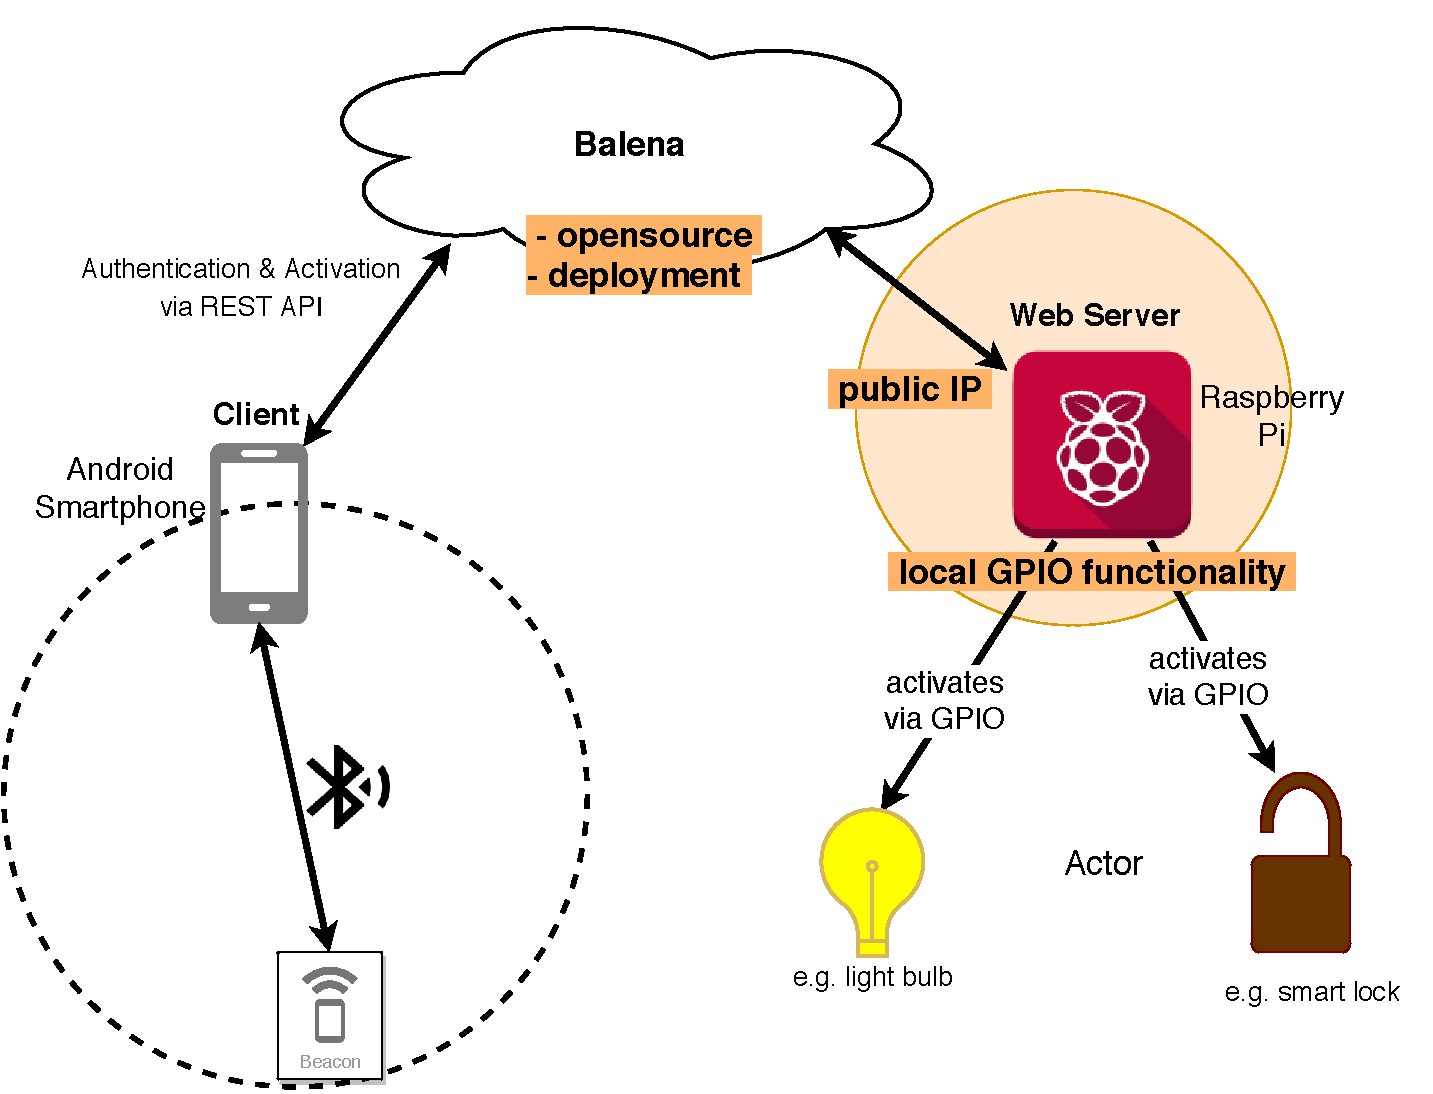
\includegraphics[width=0.99\textwidth]{Project_Architecture_final1}
	\caption{Project Architecture}
	\label{fig:projectarchitecturefinal}
\end{figure}

\section{Sensors Used}
We used mainly the Bluetooth sensor of the Android phone in order to detect the BLE beacon. Furthermore the WiFi card of the phone and Raspberry Pi were to used for communication. The GPIOs of the RaspberryPi are used for the action itself.


\section{Problems Faced}
During the project we faced various issues. Most of these were due to a lack of experience especially in terms of Android, since we both had almost zero Android experience.

\begin{enumerate}
\item 
	\begin{description}
	\item[Use of BLE Android Library] The first challenge was to find an adequate Bluetooth Library for Android, which supports the Eddystone Beacon simulated by the RaspberryPi, as well as the iBeacon provided by the chair. Once the library was selected it took quite a long time to get it working. One of the issues here were the missing errors when required Android permissions were not set. 
	\end{description}
	\item 
	\begin{description}
	\item[Background Detection on Android 8+] Prior to Android 8 it was possible to keep a service running in the background in order to detect beacons when the application is in the background. Starting with Android 8 this is not possible any more \cite{young_2017} since services are limited to running only once every 15 minutes. As a solution a new API is provided which wakes up a given application once a defined beacon is in range. Unfortunately this did not work for us, thus we were forced to keep our application permantly active by creating a persistent notification.
	\end{description}
\end{enumerate}

\section{Work Items}
Building our prototype involved various work items which we completed as follows:
\begin{enumerate}
\item 
	\begin{description}
	\item[Creating BLE Beacon] Creating a NodeJS application which serves as a BLE beacon both on the laptop and the RaspberryPi.
	\end{description}
\item 
	\begin{description}
	\item[Deployment to RaspberryPi] In order to have an easy way to deploy new versions of our application we decided to use Balena. Balena allows to run docker images on a RaspberryPi and manages the deployment.
	\end{description}
	\item 
	\begin{description}
		\item[Finding BLE Library for Android] Finding a BLE Library for Android which supports both the Eddystone beacon (RaspberryPi) and the iBeacon by the university.
	\end{description}
	\item 
	\begin{description}
		\item[Foreground Detection] Enabling the Android Application to find the beacon and then estimating the distance while being in the foreground.
	\end{description}
	\item 
	\begin{description}
		\item[Background Dectection] Enabling the Android Application to find the beacon while being in the background. In order to do this we needed to create an additional Application class which can permantly run.
	\end{description}
	\item 
		\begin{description}
		\item[RaspberyPi API] Creating an API on the RaspberryPi which interacts with the GPIOs.
	\end{description}
	\item 
		\begin{description}
		\item[Making API Requests with Android] Adding the API Request on the Android phone once the phone is near enough.
	\end{description}
		\item 
		\begin{description}
		\item[Publishing RaspberryPi API] In order to be indepent of the network setup the RaspberryPi publishes the API using a URL with localtunnel.me. Thus independently of a local network connection the API can be reached over the Internet.
	\end{description}
	\item
	\begin{description}
		\item[Testing] We used the feature branch system of Git: implementing and pushing, the other tests and merges into main branch.
	\end{description}
\end{enumerate}

\section{Work Split}

Using Git issue feature we assigned tasks to us and shared the progress with each other. Especially the merge request feature helped a lot in keeping a stable version. Overall, Philipp worked on the Beacon detection and Mehdi focused on the Android App. Testing was done by both.


\section{Concluding Remarks}
During the last months, we were able to develop a working prototype including our desired feature set. The prototype proves that such a setup is possible, however it outlines some of limitations such as battery consumptions.
Talking with Ilias during the exercises, visiting the lecture - also the guest lectures-, and working together helped us a lot to get to know new tools and possibilities of the Internet of Things world.


%----------------------------------------------------------------------------------------
%	BIBLIOGRAPHY
%----------------------------------------------------------------------------------------

\renewcommand{\refname}{\spacedlowsmallcaps{References}} % For modifying the bibliography heading

\bibliographystyle{unsrt}

\bibliography{references.bib} % The file containing the bibliography

%----------------------------------------------------------------------------------------

\end{document}